\section{Iteration 1: Decomposition of the whole system}
\label{add:it1}

\npar In the first iteration, the whole system, ReMeS is decomposed. It takes
all the requirements and quality attribute scenarios as input.

\subsection{Step 0: Confirm there is sufficient requirements information} 

% TODO de tekst in deze subsectie beschrijft niet helemaal wat in deze sectie
% moet komen. Ofwel schrappen we dit, ofwel maken we hier nog eens een overzicht
% van de requirements met prioritization door de opdrachtgever en invloed op de
% architectuur. 
% Referenced from: http://www.sei.cmu.edu/reports/06tr023.pdf

\subsection{Step 1: Identify candidate drivers}
\label{add:it1/drivers}

% TODO verwijs naar step 0?

\npar First of all when designing a decomposition for the whole system, the
choice of the drivers is very imortant since it will shape the architecture the
most. Therefore not only is the priority of the client for each quality
attribute scenario taken into account to choose the drivers, but also the impact of
that scenario on the architecure. These impacts are, together with the client
priorities, summarized in table \ref{table:add/it1/priorities}.

\begin{table}
	\begin{center}
		\begin{tabular}{| l | l | l | l | l | l | l | l | l | l |}
		\hline
		\textbf{Quality}			&	Av1	&	Av2	&	Av3	&	P1	&	P2	&	P3	&	M1	&	M2	&	M3	\\
		\hline
		\textbf{Client Priority}	&	H	&	M	&	L	&	H	&	M	&	M	&	H	&	L	&	M	\\
		\hline
		\textbf{Architecture Impact}&	L	&	H	&	L	&	H	&	H	&	M	&	M	&	L	&	M	\\
		\hline
		\end{tabular}
		\caption{An overview of all priorities which are takn into account when
		selecting the architectural drivers.}
		\label{table:add/it1/priorities}
	\end{center}
\end{table}

\npar Off course one wants to maximize the priority in both cases. Based on the
priorities in table \ref{table:add/it1/priorities}, one high priority and two
medium priority quality attribute scenarios are selected as architectural driver. An
overview of the selected drivers and their use cases is given below.

\begin{itemize}
  	\item P1 (High): Timely closure of valves
  	\begin{itemize}
  	  	\item UC8 (High) : send measurement
  		\item UC13 (High): Send alarm 
  	\end{itemize}
  	\item P2 (Medium) : Anomaly detection
  	\begin{itemize}
  	  \item UC10 (Medium) : Detect anomaly %TODO
  	\end{itemize} 
  	\item Av2 (Medium) : Missing measurements %TODO use cases ?
\end{itemize}

\npar The considered use cases includes the use cases listed below. 

\begin{itemize}
	\item UC7 (High): Send trame to remote device
	\item UC9 (High): Notify customer
	\item UC10 (Medium): Detect anomaly
\end{itemize}

\npar The choice of P1 is logical because it has the highest priority available
(both a high client priority and impact on the architecture). The reasons for
selecting P2 and Av2 are more subtle since there are still combinations
available (e.g. Av1) which precede P2 in the priority hierarchy. The choice is
twofold. First of all P2 is very easy to combine with P1 because they both place
constraints on the database access in the two different operate modi (normal and
overload). Second, the impact on the architecture is very high in contradiction
to other high (client) priority requirement such as Av1 or M1. Based on the
second argument there was also opted to go for Av2.

\npar Based on the architectural drivers, the remote module subsystem has to
provide functionality for remote module communication (receiving and sending
trames), trame storage, trame processing and stakeholder communication. 

\npar In order to obtain a better understanding of the relationships between
these functionalities, a small domain model is drafted. Figure
\ref{fig:add/it1/draft} This model can then be refined later on
in this level of decomposition.

\begin{figure}[H]
	\begin{centering}
		% TODO
		%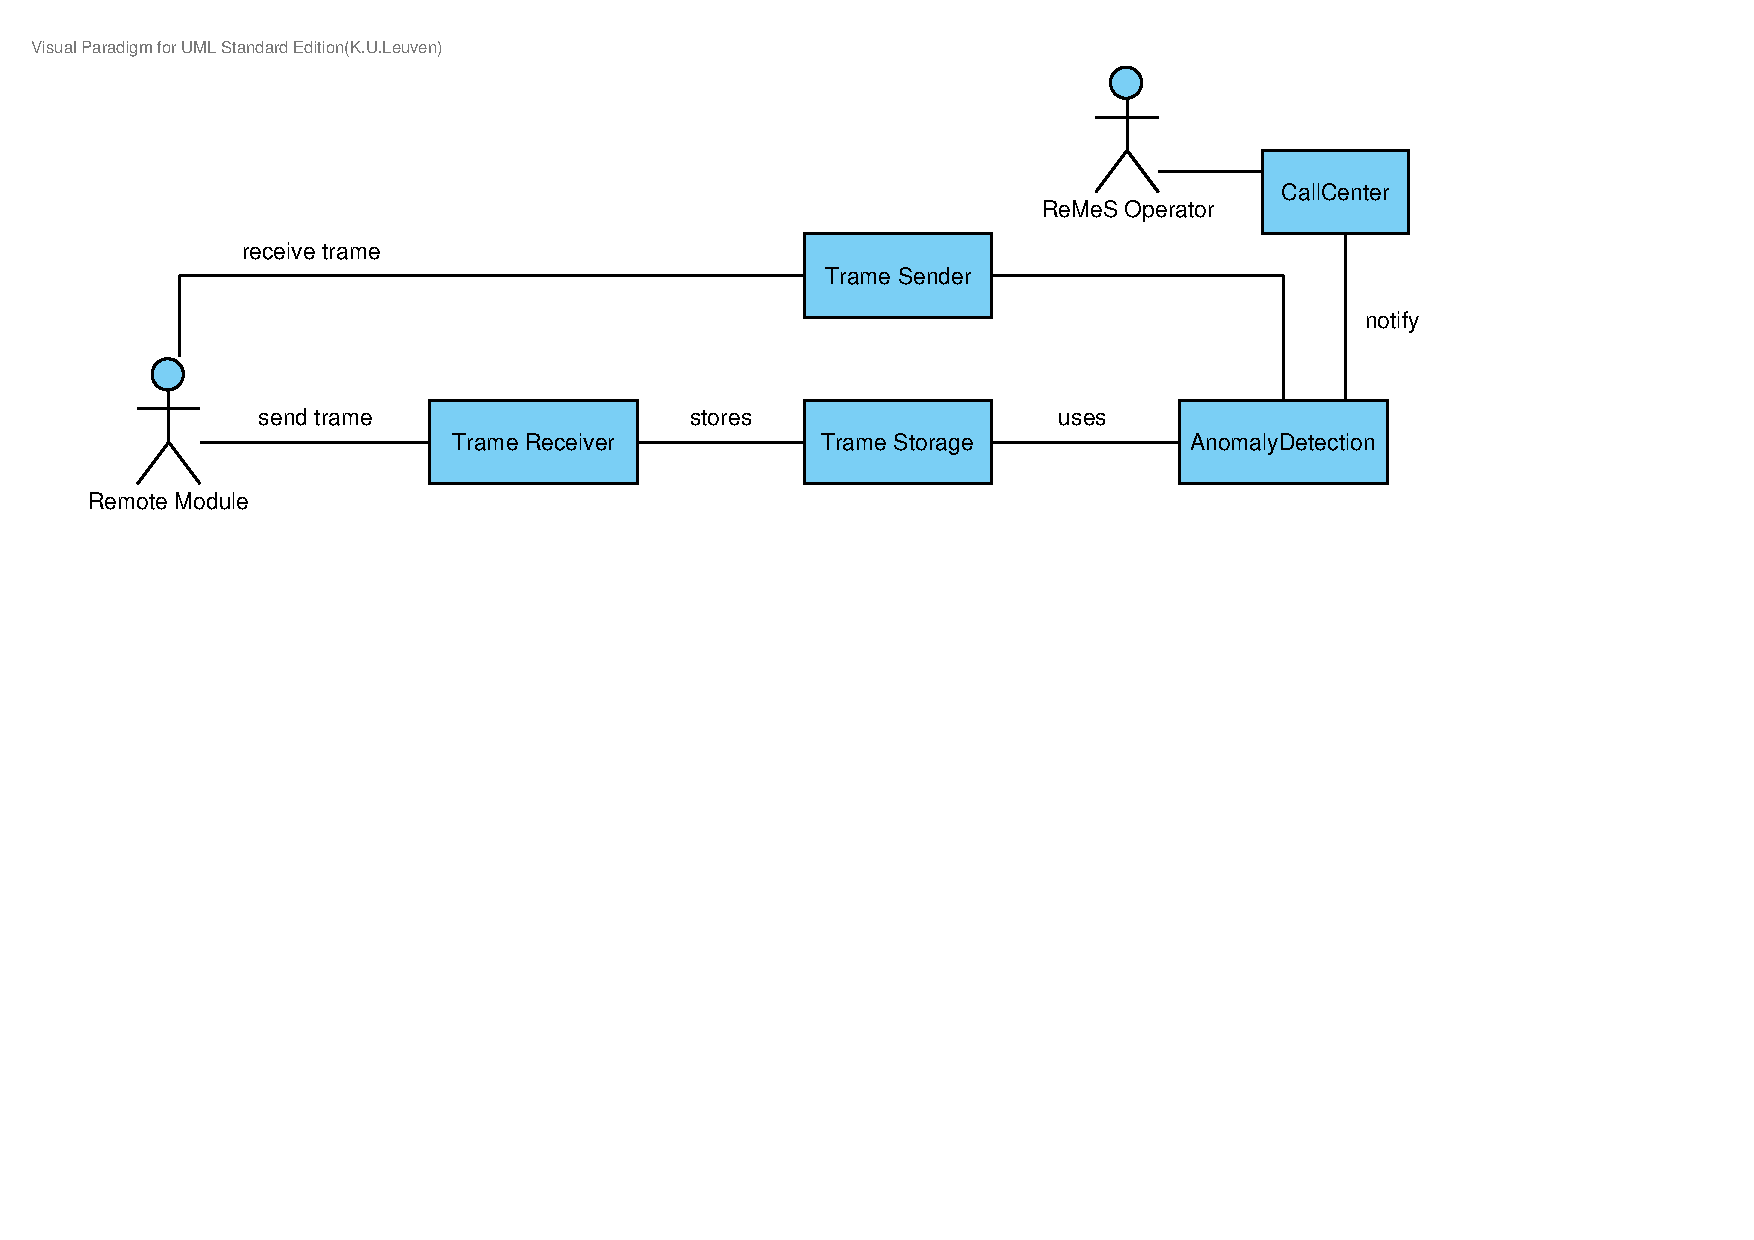
\includegraphics[width=0.6\textwidth]{figs/decomposition/whole-system/domainmodel-draft.pdf}
		\caption{Draft of the domain model used in the level 1 decomposition}
		\label{fig:add/it1/draft}
	\end{centering}
\end{figure}

\subsection{Step 2: Choose design concepts}
\label{add:it1/concepts}

\subsubsection{Tactics}
\label{add:it1/tactics}

\paragraph{Availability}
 
\npar After selecting the drivers for the current decomposition, one has to
choose the tactics to achieve them. Recall from section \ref{add:it1/drivers}
that one of the drivers was Av2. All approaches to maintain availability
involve either detection, recovery or prevention of faults.

\npar First of all, a fault needs to be detected. For this, there are three
options: ping/echo, heartbeat and exceptions. It is important to notice that the
latter is not very practical. This can be illustrated with a simple example.

\npar Suppose that a component $c_1$ depends on another component $c_2$. For
some reason, $c_1$ does not need the services of $c_2$ for a duration longer
than the detection interval of one minute (see Av2). Within this time,
no detection can occur, simply because there is no interaction between the
components. For this reason, we eliminate exceptions as a primary fault
detection system. However, exceptions will still have to be implemented in order
to make the system fail gracefully (a component being unavailable will not
cause the system to crash).

\npar Another detection method uses ping/echo. This primarily focusses on
network connectivity and will not check the availabillity of the service itself.
Again, this is not very practical. A server can be reachable, but the service on
a certain port number may be unavailable. In this case, the ping/echo
method would not detect the fault.

\npar Heartbeat on the other hand, will be part of the system itself and will be
able to check whether the service is still up and running. It will periodically
(at most every one minute) check the state of the system and send out a pulse
to a heartbeat monitor if everything is runnning fine.

\npar Another advantage of using heartbeat is that the pulse can contain data,
more specifically status data. For instance, a single failing disk in a RAID5
array can cause a warning but will not cause the system to crash. This
information can be included in the pulse of the heartbeat to inform the
administrators to replace the failing disk.

\npar As a result, heartbeat seems the best solution to detect faults.

% 
\paragraph{Performance} 

\npar For performance tactics there are three categories: resource
arbitration, resource management and resource demand.

\npar If there is more than one request to gain control over a resource, there
has to be some form of scheduling. By far the most used one is a priority
scheduler where requests are served earlier when they have a higher priority.
This is particulary useful for alarms to still reach the appropriate parties in
time even when the system is in overload mode. 

\npar Secondly there is resource management. To process more than one trame at a
time, concurrency can be introduced. This can be done in various ways. Several
threads can be started on one processor, on separate processors or even on
separate systems. Another possibilitiy is off course increasing the available
hardware but since this is not a very cost effective solution, this is left out
of consideration.

\npar On a lower level one could also try to minimize network overhead by
only sending small amounts of data in each trame. This is achieved by
limiting the size of the trames to 160 bytes.

\npar To conclude a small overview is given of all selected tactics for this
decomposition.

\begin{itemize}
 	\item Av1 (High): Measurement database Failure
 	\begin{itemize}
 		\item Detection: Heartbeat 
 		\item Recovery : Active replication
 	\end{itemize}
  	\item P1 (High): Timely closure of valves
  	\begin{itemize}
  		\item Resource arbitration : Scheduling
		\item Resource management  : concurrency
		\item Resource demand      : limited tramesize
  	\end{itemize}
\end{itemize}

\subsubsection{Design Patterns}
\label{add:it1/patterns}

\paragraph{Active Object}

\npar With respect to resource arbitration and resouce management, the
\emph{Active Object} design pattern is chosen for trame communication and
processing. Schedulers will determine the order in which trames are received,
processed and sent. 

\paragraph{Strategy}

\npar The previously mentioned schedulers will have different scheduling
policies, implemented with the \emph{Strategy} design pattern, in order to
allow operation in different modes.

\npar The trames will have to be objectified. This will yield two advantages.
Firstly, the scheduler can be implemented using the \emph{Command Processor}
design pattern. Secondly, a unified language will exist for all vendor
specific trame formats.

\paragraph{Resource Pool}

\npar To allow load balancing (and hence increase the performance) multiple
instances of the anomaly detection are created . This can be achieved by using
the \emph{Resource Pool} design pattern. 

\paragraph{Shared Repository}

\npar Since several databases will be needed in this iteration, the
\emph{Shared Repository} pattern will be employed to %TODO argumenten pro en
% contra?

\subsection{Step 3: Instantiate architectural elements and allocate responsibilities}
\label{add:it1/elements}

\begin{figure}[H]
	\begin{centering}
		% TODO Figure
		%\includegraphics[width=0.6\textwidth]{figs/decomposition/whole-system/decomposition.pdf}
		\caption{The decomposition of the Outbound Communicatin Scheduler. Iteration
		1}
		\label{fig:add/it1/decomposition}
	\end{centering}
\end{figure}

\subsubsection{Remote Module Communication unit}

\npar This module is responsible for all communication from and to remote
modules (all types of communication and both valves and control devices).
Incoming trames (from remote devices) are handed over to the storage scheduler.
Trames which need to be sent to to remote modules are dispatched to the correct
module through the correct medium.

\subsubsection{Storage Scheduler}

\npar This scheduler gets all incoming trames from remote modules and schedules
them for storage. Dependent on the active scheduling policy trames can be
prioritized over other trames. For instance, an incoming alarm trame for a gas
leak has top priority and has strict bounds on the delivery time (see the
quality attribute scenarios). Furthermore serves this scheduler as a buffer.
This is particularly useful when the storage unit is overloaded.

% \subsubsection{Heartbeat monitor cluster}
%  TODO: verplaatsen of weggooien.
% \npar The heartbeat monitor cluster is the result of the tactic to detect a
% fault, namely heartbeat. This component will monitor all other components to see
% if they are still alive (i.e. not crashed). Off course it is not unthinkable
% that the monitor component fails itself. Therefore this component has to monitor
% itself by for example an extra monitor that monitors the monitor.

\subsubsection{Storage of trames}

\npar This component is responsible for all storage of measurements (and
measurements only). It receives trames from the storage scheduler and notifies
the Anomaly Detection scheduler when a new trame is available.

\subsubsection{Anomaly Detection Scheduler}

\npar When the storage unit has stored a new trame, this scheduler is notified
and fetches the freshly stored trame. Analogous to the other scheduler this
scheduler serves as a buffer to prevent overloading on the anomaly detection
unit. Once again different scheduling policies can be switched on.

\subsubsection{Notification Unit}

\npar This module is contacted by the anomaly detection. When the latter detects
an anomaly in the usage of one the utilities of a customer or a (non false)
alarm, then that customer (and possibly the emergency services) needs to
notified. This is the responsibility of the Notification Unit.

\subsubsection{Anomaly Detection Unit}

\npar The Anomaly Detection unit is responsible for running the algorithms to
discover anomalies. It receives trames from the anomaly detection scheduler so
it can process them. After receiving such a trame, additional trames are fetched
by sending a read query to the storage scheduler. These additional trames
are from the same customer or utility company because the detection algorithms
off course work based on data sets instead of single trames. Notice that there
are multiple instances of this anomaly detection unit. This allows load
balancing, cf. P2.

\npar The task of this unit is the managing of all these instances. This
includes monitoring the load of all the instances, performing the read queries
and distributing the resulting trames. Upon detecting an anomaly two possible
actions (or both) can be undertaken. The first is sealing a valve if it is a
severe leak (this action is represented by the dependency between the outgoing
communication scheduler and the anomaly detection). The second is notifying the
approriate parties (the customer and/or the emergency services).

\subsubsection{Outgoing Communication Scheduler}

\npar The outgoing communication scheduler has as duty the scheduling of
trames which are sent to remote modules. There is a need for scheduling because
control trames to shut a valve need to reach the specified module within certain
time constraints according to P1. This scheduling can again be realized by the
use of different policies.

\subsubsection{Stakeholder Communication unit}

\npar This unit is responsible for all communication towards stakeholders (e.g.
customers, emergencyservices, etc.). 

\subsection{Step 4: Define interfaces for instantiated elements}
\label{add:it1/interfaces}

\subsubsection{Remote Module Communication Unit}

\paragraph{InputTrame} %TODO: parameter van de receive

\npar The remote module communication unit offers one method
\method{receive(\ldots)} which is invoked by remote modules whenever they want
to send a trame towards ReMeS.

\paragraph{OutputTrame}

\npar The output translator also offers only one method, \method{send(trame)}.
This method can be invoked by components who need to communicate with one or
more remote modules.

\subsubsection{Storage Scheduler}

\paragraph{StorageQueryScheduler}

\npar The \interface{StorageQueryScheduler} has one method,
\method{schedule(query)}. This method will feed the given query into the
scheduler. 

\subsubsection{Storage}

\paragraph{TrameCRUD}

\npar This interface offers four methods, summarized CRUD. This abbreviation
stands for : ``Create Read Update Delete'' and refers to the four basic
operations possible on a database.
 
\npar The first method, \method{create(query)}, can be used for the insertion of
a new data table. The \method{read(query)} method serves to read a certain
amount of trames (e.g. all measurements a of certain utility provider or
customer). Third there is an \method{update(query)} method to change the
content of a table (e.g. add a measurement for a certain customer). Finally a
\method{delete(query)} method is provided to delete data.

\subsubsection{Anomaly Detection Scheduler}

\paragraph{DetectionScheduler}

\npar The \interface{DetectionScheduler} interface offers a
\method{schedule(trame)} method which will offer the given trame to the
scheduler.

\subsubsection{Anomaly Detection}

\paragraph{AnomalyDetector}

\npar This interface once again offers only one method \method{detect(trame)}.
Invoking this method can trigger various anomaly detection algorithms to start
running (or add the given trame to an already running algoritm). There can be an
analysis for the utility provider or customer where the measurement belongs too.
These algorithms typically take more than one trame as input so additional
trames may be fetched. Therefore a read query be scheduled through the
\interface{StorageQueryScheduler} by invoking the \method{read(query)} (where
the query off course has to be constructed within the \method{detect} call).

\npar When the outcome of one or more algorithms indicates that an anomaly is
found (or when the initial trame was an alarm trame) the customer and/or emergency
services may have to be notified. Therefore the \method{send(notification)}
of the \interface{NotifyUnit} can be used. This method call will handle the
notification.

\subsubsection{Notification Unit}

\paragraph{NotifyUnit}

\npar The interface this notification unit offers, has one method, namely a
\method{send(notification)}. Invoking this method results in the notification of
the recipient (which is included in the notification parameter) with the actual
message.

\subsubsection{Outbound Remote Module Scheduler}

\paragraph{OutboundTrameScheduler}

\npar To fulfill the scheduling functionality a method is needed where
components can send their trames to. This method is called
\method{schedule(trame)} and feeds the given trame into the scheduler where it
will wait to be redirected to the communication unit.

\subsubsection{Shared Repository} 

\npar All interfaces offered by the shared repository are analogous to the
\interface{TrameCRUD} to a great extent. After all the basis of all of these
interfaces is the CRUD principle.

\paragraph{CustomerProfileCRUD}
%TODO: niet volgens CRUD principe
\npar This interface includes a \method{getCustomerByDeviceId(deviceId)} to
enable the remote communication module to retrieve the customer which belongs to
a certain incoming trame. This customer information can then be used throughout
the system whenever needed.

\paragraph{RemoteModuleConfigurationCRUD}

\npar 

\paragraph{AlarmStorageCRUD}

\npar 

\subsection{Step 5: Verify and refine}
\label{add:it1/verification}

\npar In this step, we verify that that the element decomposition thus far meets
the functional requirements and quality attribute requirements. Also, child
elements are prepared for further decomposition.

\npar Three things have to be verified. First, we will verify that all
functional requirements and quality attribute requirements of the parent element
have been allocated to one or more child elements in the decomposition.
Secondly, all responsibilities that were assigned to child modules are
translated into functional requirements for the individual items and finally,
quality attribute scenarios for individual child elements are refined if
necessary.

\npar We will list all the child elements, together with their allocated use
cases and quality attribute requirements. If a requirement is split or
delegated, it is also mentioned in the list. To conclude an overview is given of
resolved requirements in this iteration.

\begin{itemize}
	\item Communication Unit
	\begin{itemize}
	  	\item UCx : Retrieve Customer from remote module identification %TODO dit
	  	% wordt toegewezen aan communication unit, maar het is wel een oproep van
	  	% een methode op other (``getCustomerby etc)
	  	\item UCy : Retrieve Remote Module protocol
		\item UC7': Send trame to remote device (split)
		\item Av2': Missing measurements (split)
		\item M1' : Dynamic pricing (split)
		\item M2' : Fine-grained metering for enterprises (split)
		\item M3' : Decentralized electricity generation (split)
	\end{itemize}
	\item Storage Scheduler
	\begin{itemize}
		\item P1' : Timely closure of valves (split)
	\end{itemize}
	\item Storage
	\begin{itemize}
		\item Av1: Measurement database failure (delegated)
		\item Av2': Missing measurements (split)
	  	\item P3': Requests to the measurement database (delegated)
	\end{itemize}
	\item Anomaly Detection Scheduler
	\begin{itemize}
		\item UCz: Determine the operational mode (derived)
		\item P1' : Timely closure of valves (split)
	  	\item P2': Anomaly Detection (split)
	\end{itemize}
	\item Anomaly Detection
	\item Customer Communication Unit
	\begin{itemize}
		\item UC9: Notify Customer
	\end{itemize}
	\item Outgoing Communication Scheduler
	\begin{itemize}
	  \item P1' : Timely closure of valves
	\end{itemize}
	\item Other functionality
	\begin{itemize}
	  	\item UC1: Log in
	  	\item UC2: Log off
	  	\item UC3: Register customer
	  	\item UC4: Unregister customer
	  	\item UC5: Associate device to customer
	  	\item UC6: Customize customer profile
	  	\item UC11: Operate remote actuator remotely
	  	\item UC12: Set alarm recipients
	  	\item UC14: Request consumption predictions
	  	\item UC15: Generate invoice
	  	\item UC16: Mark invoice paid
	  	\item UC17: Perform research
	  	\item Av3: Third Party Billing Service failure
	  	\item M1': Dynamic pricing
	  	\item M2: Fine-grained metering for enterprises
	  	\item M3': Decentralized electricity generation
	\end{itemize}
	\item Resolved requirements
	\begin{itemize}
		\item UC7': Send trame to remote device (split)
		\item UC8 : Send measurement
		\item UC13: Send alarm
		\item UC10: Detect anomaly
		\item P1' : Timely closure of valves (split)
		\item P2' : Anomaly detection (split)
	\end{itemize}
	\item 
\end{itemize}
